\documentclass[12pt]{article}

\usepackage{natbib,amsfonts,graphics,amsmath}
\usepackage{graphicx}

%
% New command file
%

% Partial Derivative
\newcommand{\D}[2]{\frac{\partial{#1}}{\partial{#2}}}
\newcommand{\dd}[2]{\frac{d{#1}}{d{#2}}}
\newcommand{\ND}[3]{\frac{\partial^{#3}{#1}}{\partial{#2}^{#3}}}
\newcommand{\DHO}[2]{\frac{\partial^H{#1}}{\partial{#2}}}
\newcommand{\de}[2]{\frac{\delta{#1}}{\delta{#2}}}
\newcommand{\deln}[3]{\frac{\delta^#3 #1}{\delta #2^#3}}
\newcommand{\SD}[2]{\frac{\partial^2{#1}}{\partial{#2}\partial{#2}}}
\newcommand{\order}[1]{\mathcal{O}\left(#1\right)}
\newcommand{\etal}{{\it\space et al. }}
\newcommand{\ub}{\mathbf{u}}
\newcommand{\fb}{\mathbf{f}}
\newcommand{\rhobar}{\overline{\rho}}
\newcommand{\xb}{\mathbf{x}}
\newcommand{\ut}{\utilde{u}}
\newcommand{\ol}[1]{\overline{#1}}
\newcommand{\twocol}[2]{\parbox{2in}{#1}\parbox{2in}{#2}}
%
% \insertfig{scalefactor}{epsfile}{caption}{label}
%
\newcommand{\insertfig}[4]{
	\begin{figure}[ht!]
	\centerline{
	\scalebox{#1}{\includegraphics{#2}}
	}
	\caption{#3}
	\label{#4}
	\end{figure}}


\begin{document}

\title{Derivation of the nondimensional lee wave equations}

\author{Oliver Fringer}

\maketitle

\section{Dimensional analysis}

The form drag $F$ (per unit width) due to a hill of height $h_0$ in an infinitely 
deep fluid is characterized by the dimensional quantities
$U$, $k$, $N$, and $h_0$.  Choosing $U$ and $N$ to nondimensionalize $k$ and $h_0$, the governing
nondimensional parameters are $J = N h_0/U$ and $\epsilon = k U/N$.  Since the units of the form drag
are length$^3$~time$^{-2}$, then a scale for $F$ in terms of $U$ and $N$ is $\rho_0 U^3 N^{-1}$. Therefore,
the form drag must satisfy
\[
\frac{F}{\rho_0 U^3 N^{-1}} = f(J, \epsilon)\,.
\]

\section{Nondimensional equations} \label{eq:equations}

Let $\ub_{\mbox{total}} = U {\bf e}_x + \ub$, $\rho_{\mbox{total}} = \rhobar(z) + \rho$, and
$p_{\mbox{total}} = \rho_0 \overline{p}(z) + \rho_0 p$ (the total notation is
to avoid carrying around the prime, but in a paper you should carry around the prime).
The steady momentum and density transport equations are given by
\begin{eqnarray}
U \D{u}{x} + \ub\cdot\nabla u &=& -\D{p}{x}\,,\\
U \D{w}{x} + \ub\cdot\nabla w &=& -\D{p}{z} - \frac{\rho}{\rho_0} g\,,\\
U \D{\rho}{x} + \ub\cdot\nabla\rho &=& \frac{\rho_0 N^2}{g} w\,,
\end{eqnarray}
where $N^2 = -g/\rho_0 \partial\rhobar/\partial z$, subject to continuity $\nabla\cdot\ub=0$ and
the kinematic bottom boundary condition
\[
U\D{h}{x} + u \D{h}{x} = w\,.
\]  
Nondimensionalize with
\begin{eqnarray*}
u &=& u_0 u^*\,,\\
w &=& w_0 w^*\,,\\
\rho &=& R \rho^*\,,\\
p &=& P p^*\,,\\
x &=& k^{-1} x^*\,,\\
z &=& \delta z^*\,.
\end{eqnarray*}
Nondimensionalizing the kinematic bottom boundary condition gives
(after ignoring the $*$)
\[
k U h_0 \D{h}{x} + k u_0 h_0 \D{h}{x} = w_0 w\,.
\]
If we require a balance between the linear terms, this implies $w_0 = k h_0 U$, so that
\[
\D{h}{x} + F \D{h}{x} = w\,,
\]
where $F = u_0/U$ is a Froude number. Now, the vertical scale of the flow as given by $\delta$ is not the
same as the hill height $h_0$, since $\delta$ must be finite as $h_0\to 0$ (the linear limit). The 
vertical scale is thus dictated by continuity, which requires
\[
k u_0 \D{u}{x} + \frac{w_0}{\delta} \D{w}{z} = 0\,,
\]
or, since this implies $k u_0 = w_0/\delta$, then we must have $\delta = w_0/(k u_0) = k h_0 U/(k u_0) = F^{-1} h_0$.
Nondimensionalizing the $u$-momentum equation,
\begin{eqnarray}
k u_0 U \D{u}{x} + k u_0^2\ub\cdot\nabla u  &=& -k P \D{p}{x}\,.
\end{eqnarray}
Since we require a leading-order balance between the pressure gradient and the linear momentum advection term,
we must have $P = u_0 U$, which gives
\begin{eqnarray}
\D{u}{x} + F \ub\cdot\nabla u &=& -\D{p}{x}\,.
\end{eqnarray}
The nondimensional density transport equation is given by
\[
k U R \D{\rho}{x} + k u_0 R \ub\cdot\nabla\rho = \frac{k \rho_0 h_0 N^2 U}{g} w\,.
\]
If we require a balance between the linear advection terms, then the scale for the density
perturbation is 
\[
R = \frac{\rho_0 N^2 h_0}{g}\,,
\]
so that the nondimensional density equation is
\[
\D{\rho}{x} + F \ub\cdot\nabla\rho = w\,.
\]
Nondimensionalizing the vertical momentum equation, we have
\[
k^2 h_0 U^2 \D{w}{x} + k^2 h_0 u_0^2\ub\cdot\nabla w = -\frac{P}{\delta}\D{p}{z} - \frac{g R}{\rho_0} \rho\,.
\]
If we require a vertical hydrostatic balance to leading order, then we must have 
\[
\frac{P}{\delta} = \frac{g R \delta}{\rho_0} 
  = N^2 h_0\,,
\]
and
\[
P = \frac{g R \delta}{\rho_0} 
  = \frac{g}{\rho_0} \frac{\rho_0 N^2 h_0}{g} \frac{h_0}{F}
  = \frac{g}{\rho_0} \frac{\rho_0 N^2 h_0}{g} \frac{U}{N}
  = U N h_0\,.
\]
which gives
\[
\epsilon^2 \left(\D{w}{x} + F\ub\cdot\nabla w\right) = -\D{p}{z} - \rho\,,
\]
where 
\[
\epsilon = \frac{k U}{N}
\]
is the nonhydrostatic parameter. Now, returning to the pressure, since from the vertical momentum equation we
require $P = U N h_0$ and from the horizontal momentum equation we require $P = u_0 U$, then equating the
two implies that $u_0 = N h_0$ and the Froude number is given by
\[
F = \frac{u_0}{U} = \frac{N h_0}{U} = J\,,
\]
where
\[
J = \frac{N h_0}{U}\,.
\]
Therefore, in terms of $J$, the governing nondimensional equations are given by
\begin{eqnarray*}
\D{u}{x} + J\ub\cdot\nabla u &=& -\D{p}{x}\,,\\
\epsilon^2 \left(\D{w}{x} + J\ub\cdot\nabla w\right) &=& -\D{p}{z} - \rho\,,\\
\D{\rho}{x} + J \ub\cdot\nabla\rho &=& w\,,
\end{eqnarray*}
subject to $\nabla\cdot\ub=0$ and the kinematic bottom boundary condition
\[
\left(1 + J u\right)\D{h}{x} = w\,.
\]
These nondimensional equations are consistent with the original nondimensionalization which implied
that the problem is uniquely characterized by $\epsilon$ and $J$.
The relevant scales (nondimensionalized by $N$ and $U$) are given by
\begin{eqnarray*}
\frac{u_0}{U} &=& J\,,\\
\frac{w_0}{U} &=& \epsilon J\,,\\
\frac{gR}{\rho_0 U N} &=& J\,,\\
\frac{P}{U^2} &=& J\,,\\
\frac{\delta N}{U} &=& 1\,.
\end{eqnarray*}

Contrary to what is stated in the literature, we can show that it is
in fact appropriate to refer to $J$ as an internal Froude number. If we define
$Fr_\delta = u_0/\sqrt{g' \delta}$, where $g'\delta =g R/\rho_0 \delta = J U^2$, this gives
$Fr_{\delta} = J^{1/2}$. Therefore, $J^{1/2}$ can be thought of as 
the ratio of the inertial to gravitational forces arising from the perturbed
flow above the hill. Although we would expect a larger $N$ to block the flow and
reduce the magnitude of the perturbation above the hill, the scaling shows that
$u_0 = J U$, implying that the perturbation velocity above the sill increases with
increasing $J$. However, the gravitational force resulting from the perturbation is
given by $\sqrt{g'\delta} = J^{1/2} U$, which grows more slowly than $u_0$ with
increasing $J$.

\section{Linear, nonhydrostatic equations}

The governing equations in the linear limit $J\to 0$ are given by
\begin{eqnarray*}
\D{u}{x} &=& -\D{p}{x}\,,\\
\epsilon^2 \D{w}{x} &=& -\D{p}{z} - \rho\,,\\
\D{\rho}{x} &=& w\,.
\end{eqnarray*}
The governing equation for $w$ is then given by
\[ 
\ND{w}{z}{2} + \epsilon^2 \ND{w}{x}{2} + w = 0\,.
\]
Assume a sinusoidal topography such that $h(x) = \sin(x)$.

\subsection{Propagating solution}

When $\epsilon<1$, the hydrostatic solution is of the form
$w(x,z) = \cos(x + m z)$, which implies $m = (1-\epsilon^2)^{1/2}$.  Substitution into
the governing linear equations gives
\begin{eqnarray*}
u(x,z) &=& -m \cos(x + m z)\,,\\
w(x,z) &=& \cos(x + m z)\,,\\
\rho(x,z) &=& \sin(x + m z)\,,\\
p(x,z) &=& m \cos(x + m z)\,.
\end{eqnarray*}
The dimensional form drag (per unit width) over one wavelength is given by (here, $*$ implies dimensional
quantities)
\[
F^* = \int_{0}^{2\pi/k^*} p^*(x^*,z^*=0)\D{h^*}{x^*}\, dx^*\,.
\]
Nondimensionalizing gives
\[
\frac{F^*}{\rho_0 U^3 N^{-1}} = J^2 \int_{0}^{2\pi} p(x,z=0)\D{h}{x}\, dx\,.
\]
Substitution of $p$ and $h$ then gives
\[
\frac{F^*}{\rho_0 U^3 N^{-1}} = \pi J^2\left(1 - \epsilon^2\right)^{1/2}\,.
\]


\subsection{Evanescent solution}

When $\epsilon>1$, the nonhydrostatic solution is of the form
$w(x,z) = \cos(x)\exp(-m z)$, which implies $m = (\epsilon^2-1)^{1/2}$.  Substitution into
the governing linear equations gives
\begin{eqnarray*}
u(x,z) &=& m \sin(x) \exp(-m z)\,,\\
w(x,z) &=& \cos(x) \exp(-m z)\,,\\
\rho(x,z) &=& \sin(x) \exp(-m z)\,,\\
p(x,z) &=& -m \sin(x) \exp(-m z)\,.
\end{eqnarray*}
Since $p$ and $w$ are $\pi/2$ out of phase, the form drag is identically zero.

\subsection{Perturbation expansion}

Representing the vertical displacement of a streamline intersecting the point $(x,z)$ from its upstream position as 
\[
\delta(x,z) = z-z_o,
\]
we can recast equations 1-3 into Long's Model (Long 1953)
\[
\nabla^2\delta + \frac{N^2}{U^2}\delta = 0.
\]
Upon taking the hydrostatic approximation, this simplifies further to
\[
\partial_z^2\delta + l^2\delta = 0,
\]
where the subscript z represents differentiation with respect to z and $l=\frac{N}{U}$.
Assuming sinusoidal topography of the form $h(x) = h_0 cos(kx)$, the kinematic boundary condition now reads
\[
\delta(x,h(x)) = h(x) = h_0 cos(kx).
\]
We are now in a position to consider a perturbation solution for $\delta$, as in Smith 1977. We can postulate a perturbation expansion of $\delta$ in powers of J as
\[
\delta(x,z) = \delta_0+ J\delta _1 +  J^2 \delta_2+ O(J^3).
\]
And we can write the bottom boundary condition as a Taylor expansion around $x=0$ (I have foreseen the scaling $h(x)\propto h_0$ and $\partial_z \propto N/U$)
\[
\delta(x,h(x)) = \delta(x,0) + h \partial_z \delta |_0 +  h^2 \partial_z^2 \delta |_0 + O(J^3) = h(x).
\]
The 0th order solution comes rapidly upon plugging the perturbation expansion into the boundary condition
\begin{eqnarray*}
	\delta &=& \delta_0 + O(J) \\
	\delta(x,0) + O(J) &=& h(x)\\
	\implies \delta_0|_0 &=& h_0cos(kx)
\end{eqnarray*}
And, unsurprisingly, upon appeal to Long's Model, the 0th order solution for $\delta$ emerges as
\[
\delta = h_0cos(kx+lz)  + O(J).
\]
By similar steps, Smith arrived at the 1st order solution
\begin{eqnarray*}
	\delta &=& \delta_0 + J\delta_1 + O(J^2) \\
	\delta(x,0) + h \partial_z \delta |_0 +  O(J^2) &=& h(x)\\
	\delta_0|_0 +  h \partial_z \delta_0 |_0 + J\delta_1|_0 +O(J^2)&=& h(x)\\
	and \   \delta_0|_0 &=& h(x) \\
	\implies h \partial_z \delta_0 |_0 &=& -J\delta_1|_0\\
	h_0 cos(kx) \partial_z(h_(cos(kx+lz))|_0&=& -J\delta_1|_0\\
	 -J h_0 cos(kx)sin(kx) &=& -J\delta_1|_0\\
	  -J h_0 \frac{1}{2}sin(2kx) &=& -J\delta_1|_0\\
	\implies \delta_1|_0 &=& \frac{h_0}{2}sin(2kx)
\end{eqnarray*}
And, on appeal to Long's Model, we have 
\[
\delta(x,z) = h_0cos(kx+lz) + \frac{J h_0}{2}sin(2kx) + O(J^2)
\]
With a little more paper and time, it can be shown by identical steps that the 2nd order solution is  
\[
\delta(x,z) = h_0cos(kx+lz) + \frac{J h_0}{2}sin(2kx+lz) + \frac{J ^2h_0}{2}cos(kx+lz) + O(J^3)
\]
However, all of these solutions are evaluated at the displaced streamline height $z$, rather than the undisturbed height of the streamline far upstream, $z_0$. The two are related via
\[
\delta(x,z) = \delta(x,z_0+\eta(x,z_0)) = \eta(x,z_0)
\]
We can now use $\eta(x,z_0)$ to write $\delta(x,z)$ as a Taylor expansion around $z_0$, and after some effort, arrive at the 2nd order solution for $\eta(x,z_0)$:
\begin{eqnarray*}
\eta(x,z_0) &=& h_0cos(kx+lz_0)\\
 &+&\frac{1}{2}Jh_0(sin(2kx+lz_0)_ - sin(2kx + 2lz_0))\\
 &+&\frac{1}{2}J^2h_0[cos(kx+lz_0)+cos(kx+lz_0)cos(2kx+lz_0)\\
 &-&sin(kx+lz_0)sin(2kx+lz_0)+sin(kx+lz_0)sin(2kx+2lz_0)\\
 &-&2cos^2(kx+lz_0)]\\
 &+& O(J^3h_0)
\end{eqnarray*}
Note that this is an extension of Smith 1977, in which the solution is given only to $O(Jh_0)$. 

Plots of these solutions for J=0.3 are given below, as well as those of the velocity fields $u$ and $w$ that these displacements entail. Note the steepening of the streamlines increases with the order of the solution. 

Vertical streamlines imply wave breaking (Long 1953, Miles 1969) which results in heavy water pooling in valleys and reduced wave amplitude (Kimura and Manins 1980). The condition of vertical streamlines can be expressed mathematically as $\partial_z \delta = 1$. Thus I also include a plot of the maximum value of $\partial_z \delta$ as a function of J for each order solution. As Smith reported in 1977, the 1st order accurate solution for $\delta$ predicts that wave breaking will commence at $J=0.75$. With our next order solution, this threshold drops to $J=0.65$. Of course, neither solutions are suitable for analysis of such nonlinear flow; in order to limit the error in a $J=0.65$ solution to less than $5\%$, we would need a 6th order accurate expansion ($0.65^7 = 0.049$).

\begin{figure}
	\centering
	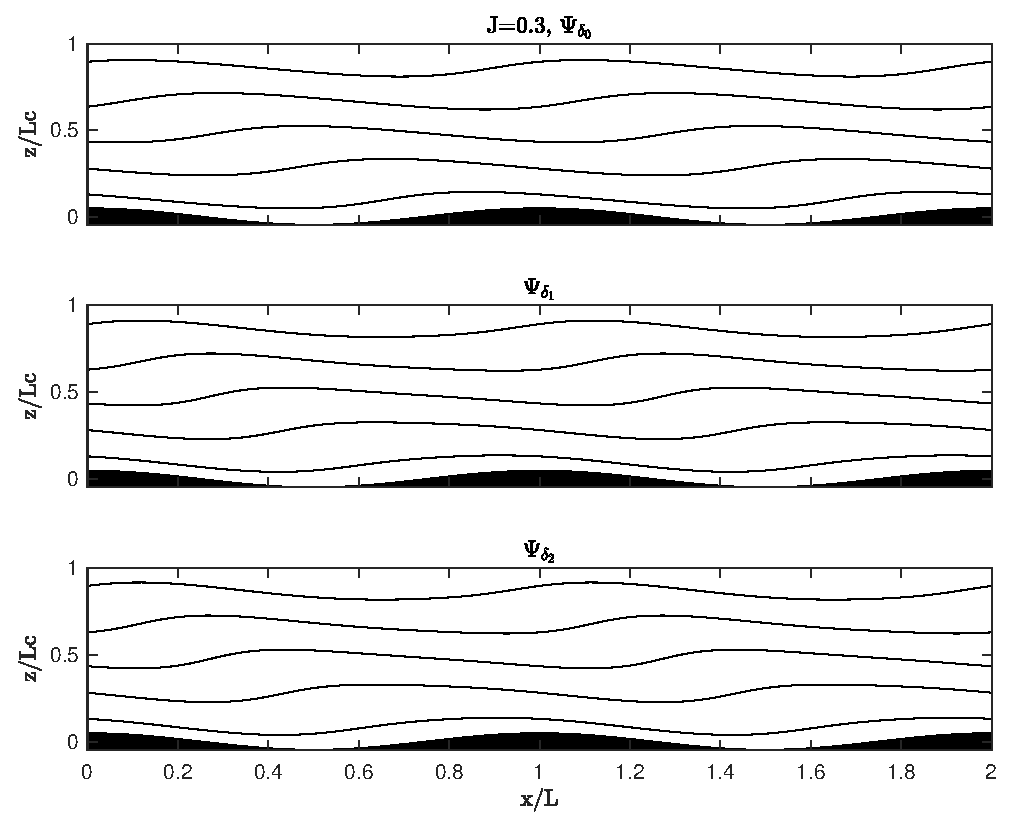
\includegraphics[width=1\textwidth]{delta_solutions.eps}
	\caption{0th, 1st, and 2nd order solutions for $\delta(x,z)$ with $J=0.3$.}
\end{figure}

\begin{figure}
	\centering
	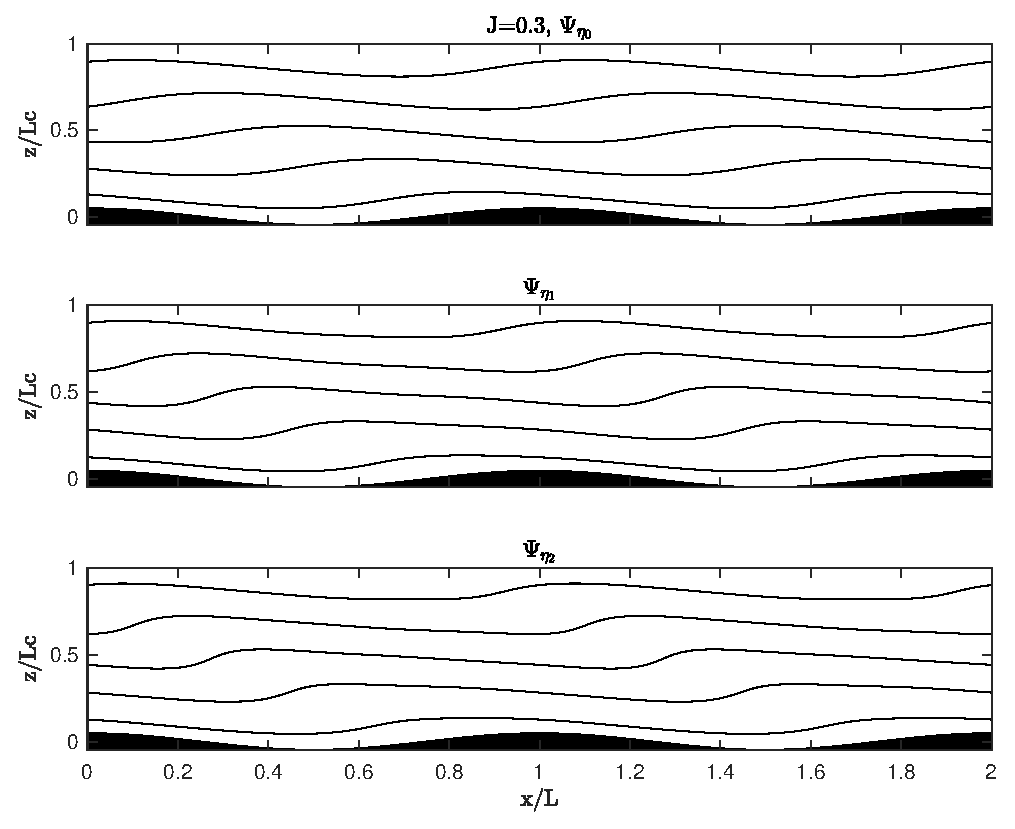
\includegraphics[width=1\textwidth]{eta_solutions.eps}
	\caption{0th, 1st, and 2nd order solutions for $\eta(x,z_0)$ with $J=0.3$.}
\end{figure}

\begin{figure}
	\centering
	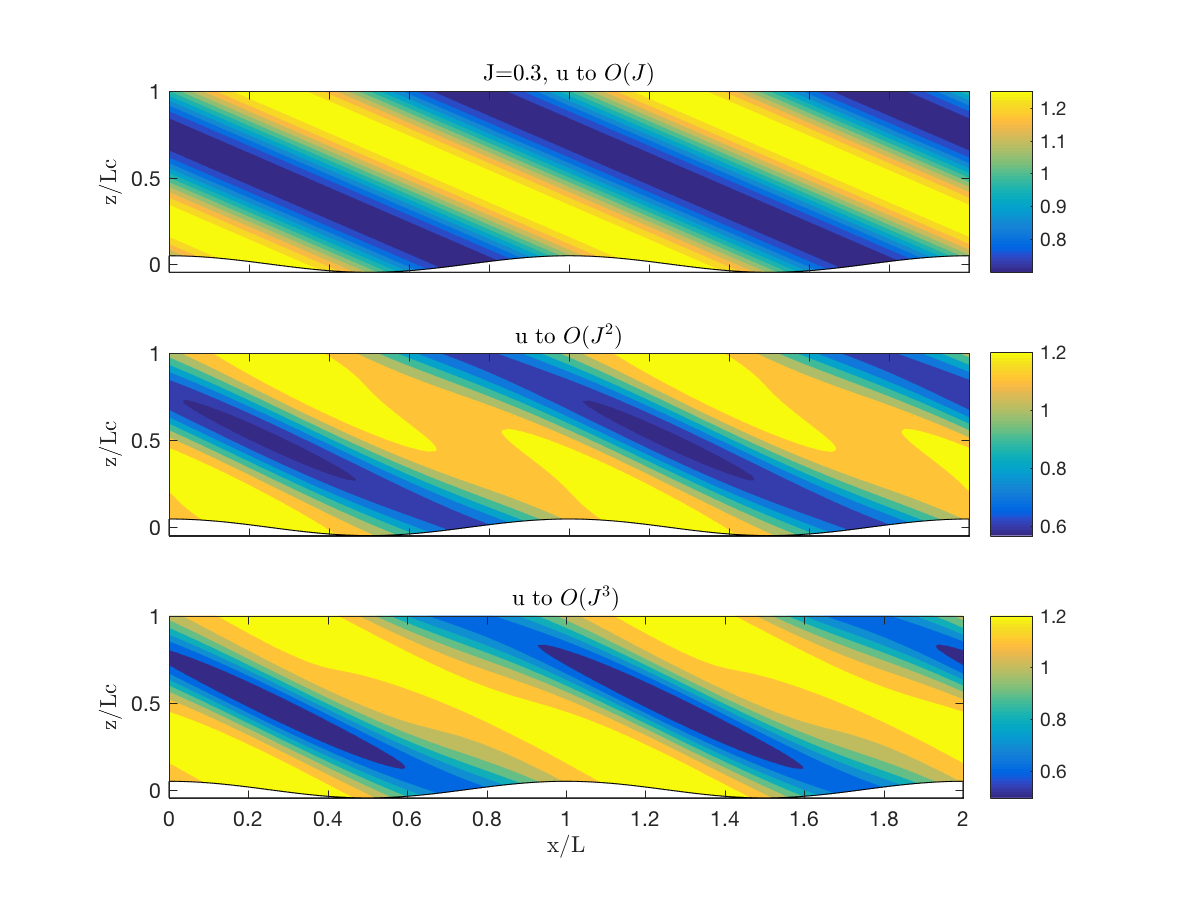
\includegraphics[width=1\textwidth]{u_solutions.eps}
	\caption{0th, 1st, and 2nd order solutions for $u(x,z_0)$ with $J=0.3$.}
\end{figure}

\begin{figure}
	\centering
	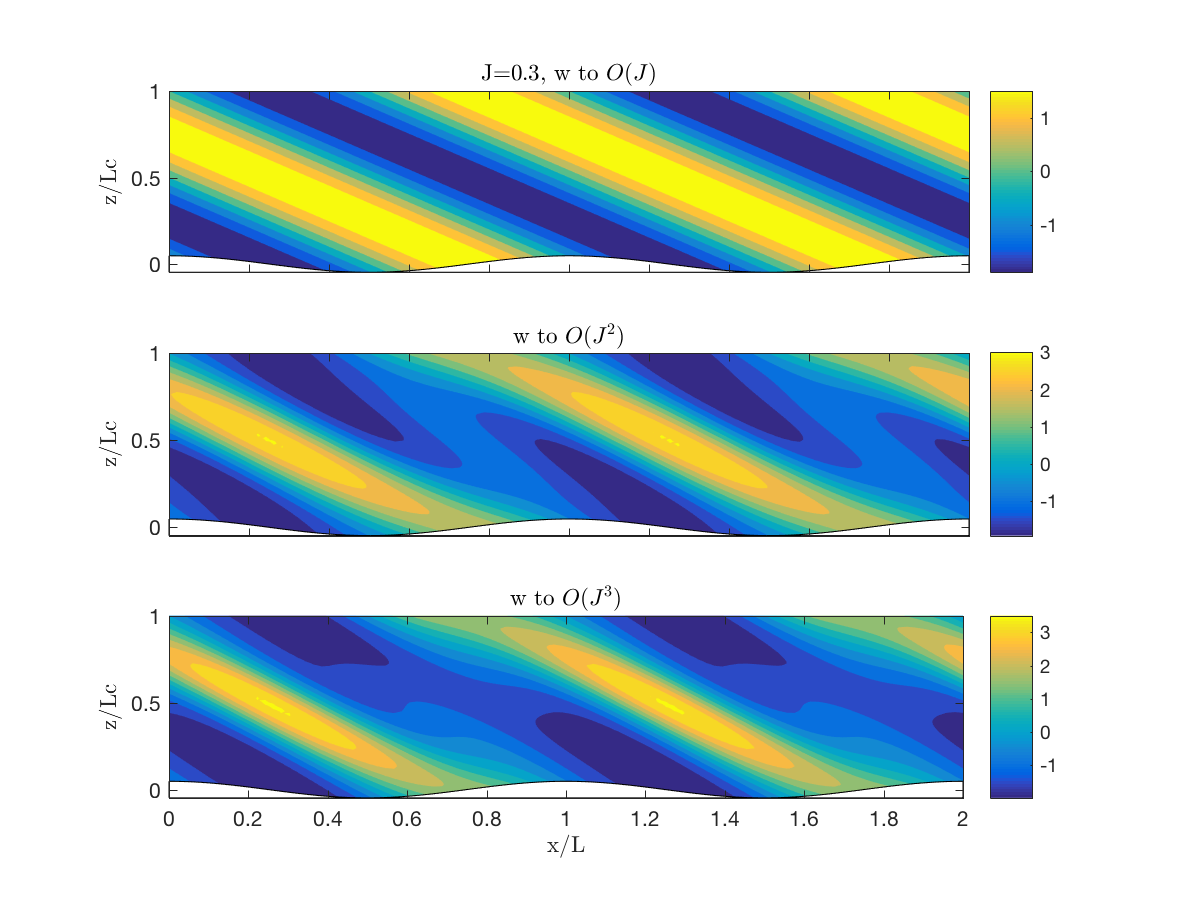
\includegraphics[width=1\textwidth]{w_solutions.eps}
	\caption{0th, 1st, and 2nd order solutions for $w(x,z_0)$ with $J=0.3$.}
\end{figure}

\begin{figure}
	\centering
	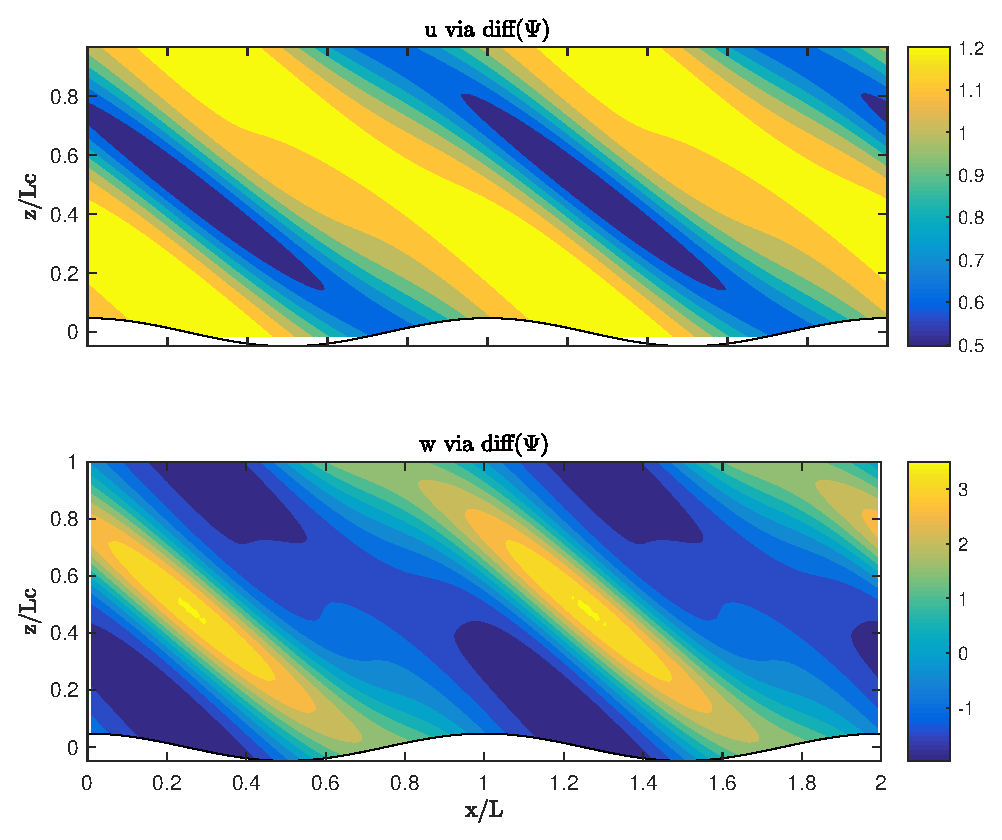
\includegraphics[width=1\textwidth]{vel_via_diff.eps}
	\caption{2nd order solutions for velocity calculated by numerical differentiation of $eta_2$.}
\end{figure}

\begin{figure}
	\centering
	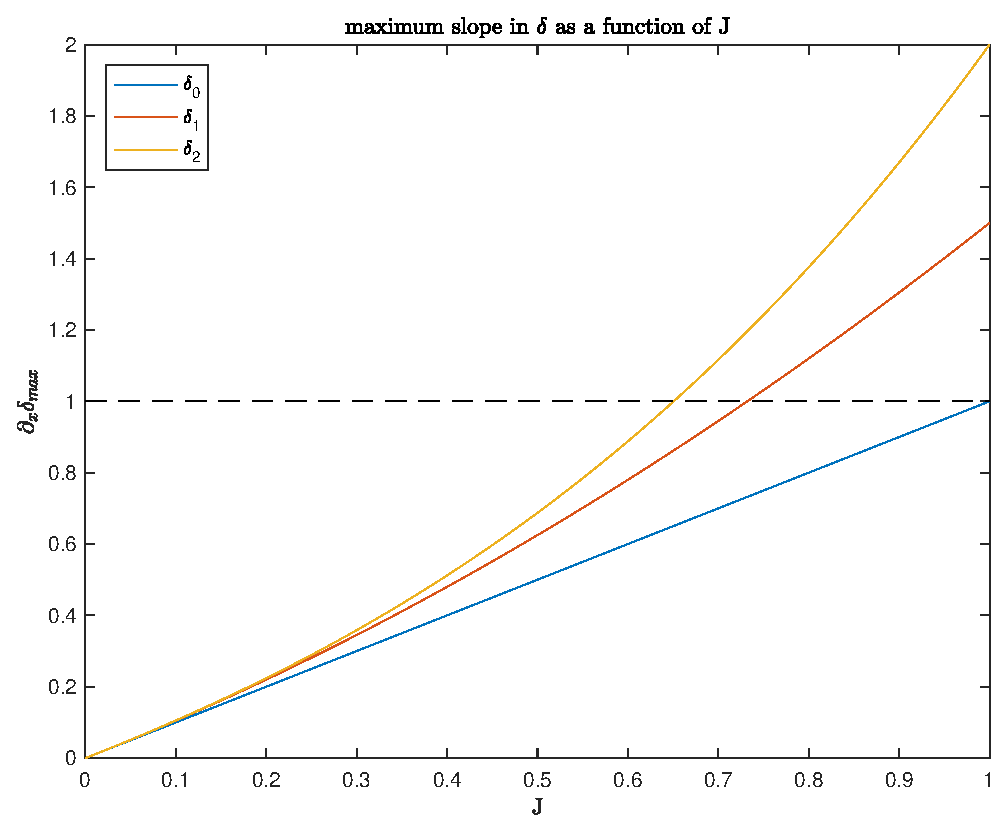
\includegraphics[width=1\textwidth]{max_slopes.eps}
	\caption{Maximum slope in $\delta$ as a function of J.}
\end{figure}

\end{document}




w = cos(x)exp(-m z)
wx = -sin(x)exp(-m z)
ux = -wz = m cos(x) exp(-m z)
u = m sin(x) exp(-m z)

rhox = w = cos(x)exp(-m z)
rho = sin(x)exp(-m z)

e2 wx = -pz - rho
pz = -e2 wx - rho = e2 sin(x) exp(-m z) - sin(x) exp(-m z) = m^2 sin(x) exp(-m z)
p = (-1/m) m^2 sin(x) exp(-m z) = -m sin(x) exp(-m z)



